\documentclass[10pt,a4paper]{report}
\usepackage[utf8]{inputenc}
\usepackage[spanish]{babel}
\usepackage[T1]{fontenc}
\usepackage{textcomp}
\usepackage{amsmath}
\usepackage{amsfonts}
\usepackage[framed,numbered,autolinebreaks]{mcode}
\usepackage{amssymb}
\usepackage{graphicx}
\usepackage{caption}
\usepackage{subcaption}
\usepackage{fancyhdr}
\usepackage{float}
\usepackage{color}
\usepackage{mcode}
\usepackage[left=2cm,right=2cm,top=2cm,bottom=2cm]{geometry}

\author{Alamilla Ortiz Cesar Alejandro\\Cabrera López Óscar Emilio\\Castillo Cruz Heriberto\\Cuevas Mondragón Ricardo\\Equipo 9}
\title{Serie 1}

\pagestyle{fancy}
\fancyhf{}
\lhead[]{}
\chead[]{}
\rfoot{\thepage}
\lfoot[]{}
\cfoot[]{}

\renewcommand\headrule
{{\color[RGB]{98,36,35}%
    \hrule height 2pt
    width\headwidth
    \vspace{1.3pt}%
    \hrule height 1pt
    width\headwidth
  }}
  \addto\captionsspanish{\def\tablename{Tabla}}%imprime Tabla en lugar de Cuadro
  %%
  \spanishdecimal{.}


\begin{document}
\thispagestyle{fancy}
\maketitle
\tableofcontents
\newpage
\setcounter{chapter}{1}

\section{Ejercicio 1}

Obtenga una expresión en términos de funciones singulares la señal de tiempo continuo x(t) mostrada en la \texttt{figura 1.1}. Utilice la parábola $u_{-3}(t)$.

\begin{figure}[H]
  \begin{center}
    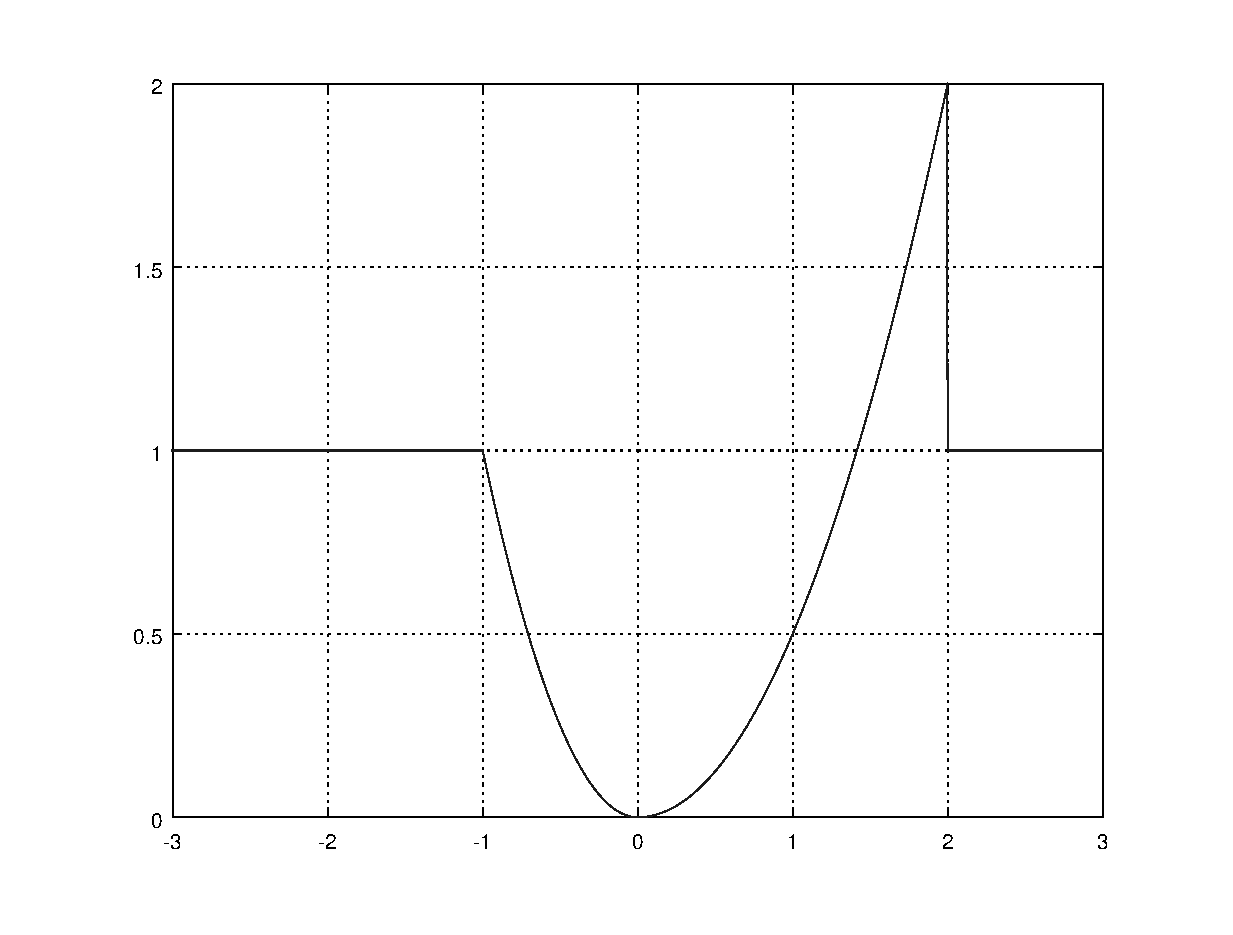
\includegraphics[width=0.5\textwidth]{./Ejercicio1/SignalEjemplo}
    \caption{Ejercicio 1}
    \label{fig:Ejercicio 1}
  \end{center}
\end{figure}

Si recordamos que la señal parábola unitaria se define como:

\[ u_{-3}(t) = \left\{
              \begin{array}{lc}
                \frac{t^2}2&t\geq0\\
                0&t<0
              \end{array}
            \right.  \]

Notaremos que la señal esta formada con la suma de dos parábolas unitarias, la primera de ellas invertida en el tiempo y ampliada por un factor de 2, la segunda no sufre ninguna transformación.

\begin{figure}[H]
  \begin{center}
    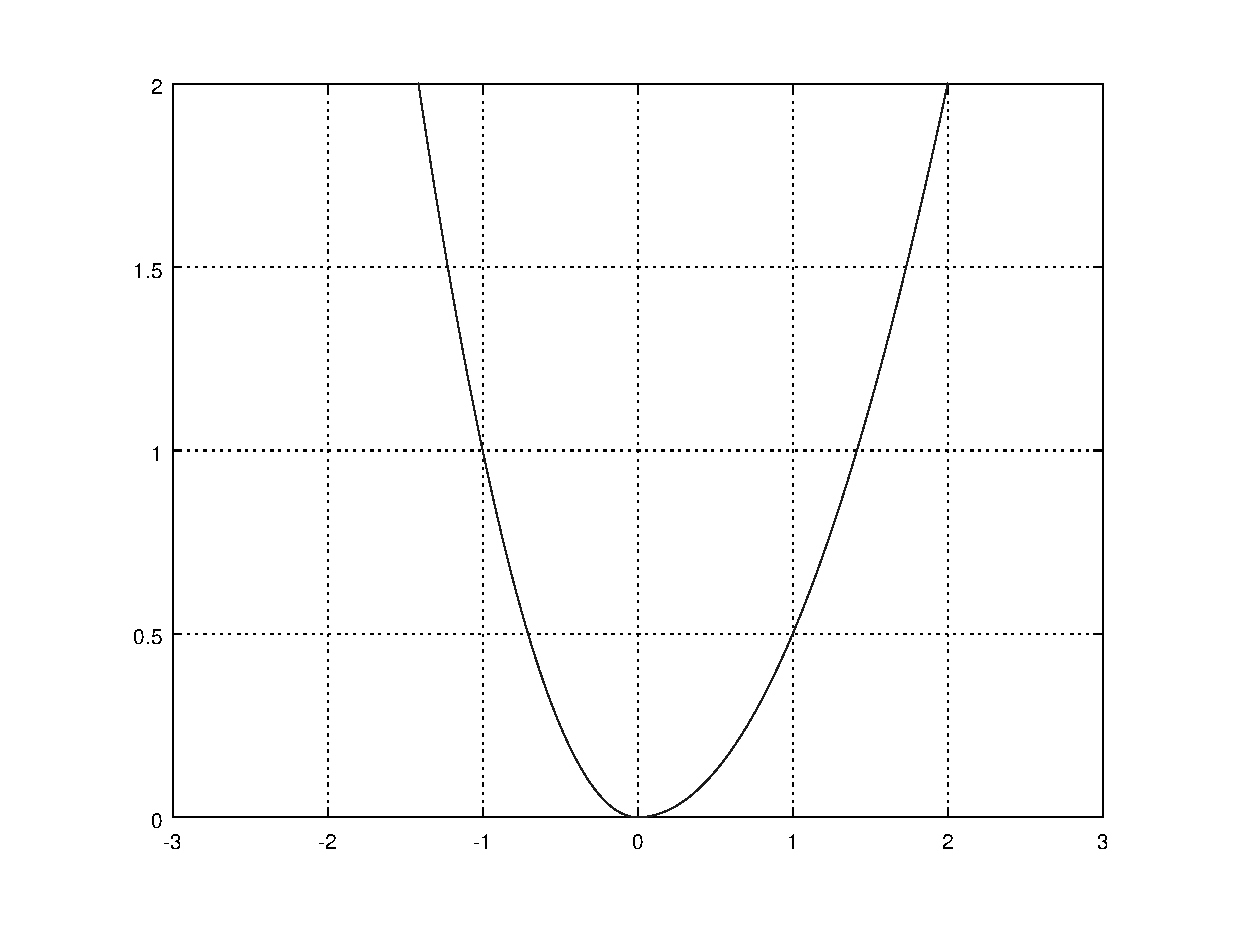
\includegraphics[width=0.6\textwidth]{./Ejercicio1/Aproximacion1}
    \caption{Primer aproximación a la señal}
    \label{fig:Aprox1}
  \end{center}
\end{figure}

Código en matlab:

\lstinputlisting{./Ejercicio1/aprox1.m}

Vemos que esta señal se acerca a la mostrada en la \texttt{figura 1.1} pero debemos limitarla a los lados desde $ -1 $ hasta $2$ esto lo conseguimos multiplicando la señal anterior con la señal $\Pi$ definida como:

\[ \Pi(t) = \left\{
              \begin{array}{lc}
                1&\left|t\right|<\frac12\\
                0&\left|t\right|>\frac12
              \end{array}
            \right. \]

Ésta señal debe ser expandida 3 veces y retrasada media unidad (consideremos que la función $\Pi$ expandida 3 veces  valdría $1$ desde $-1.5$ hasta $1.5$ y $0$ para cualquier otro valor).

\begin{figure}[H]
  \begin{center}
    
    \begin{subfigure}{0.5\textwidth}
      \begin{center}
        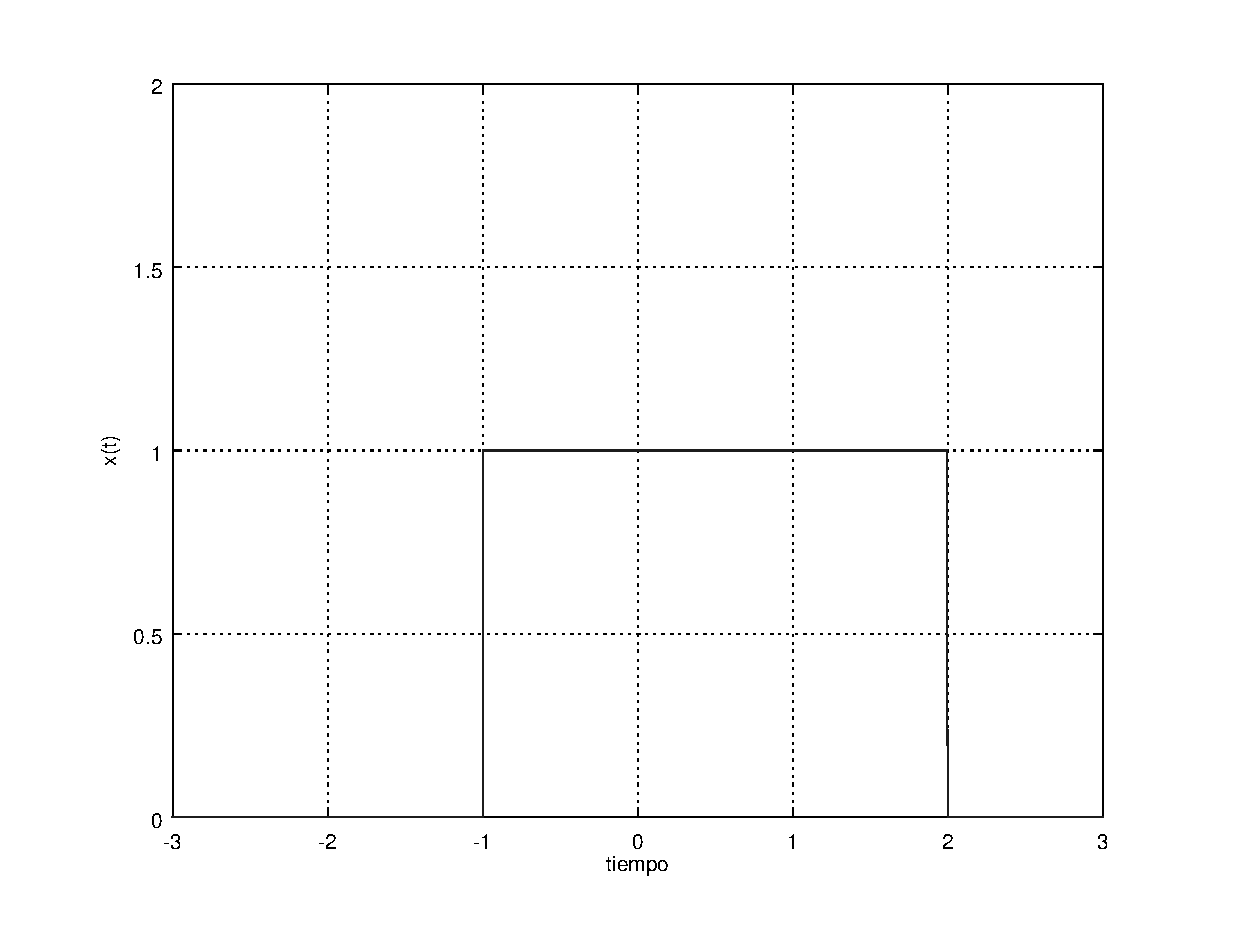
\includegraphics[width=1\linewidth]{./Ejercicio1/Aproximacion2a}
        \caption{Señal $\Pi(t)$ expandida y retrasada}
        \label{fig:Aprox2a}
      \end{center}
    \end{subfigure}%    
    \begin{subfigure}{0.5\textwidth}
      \begin{center}
        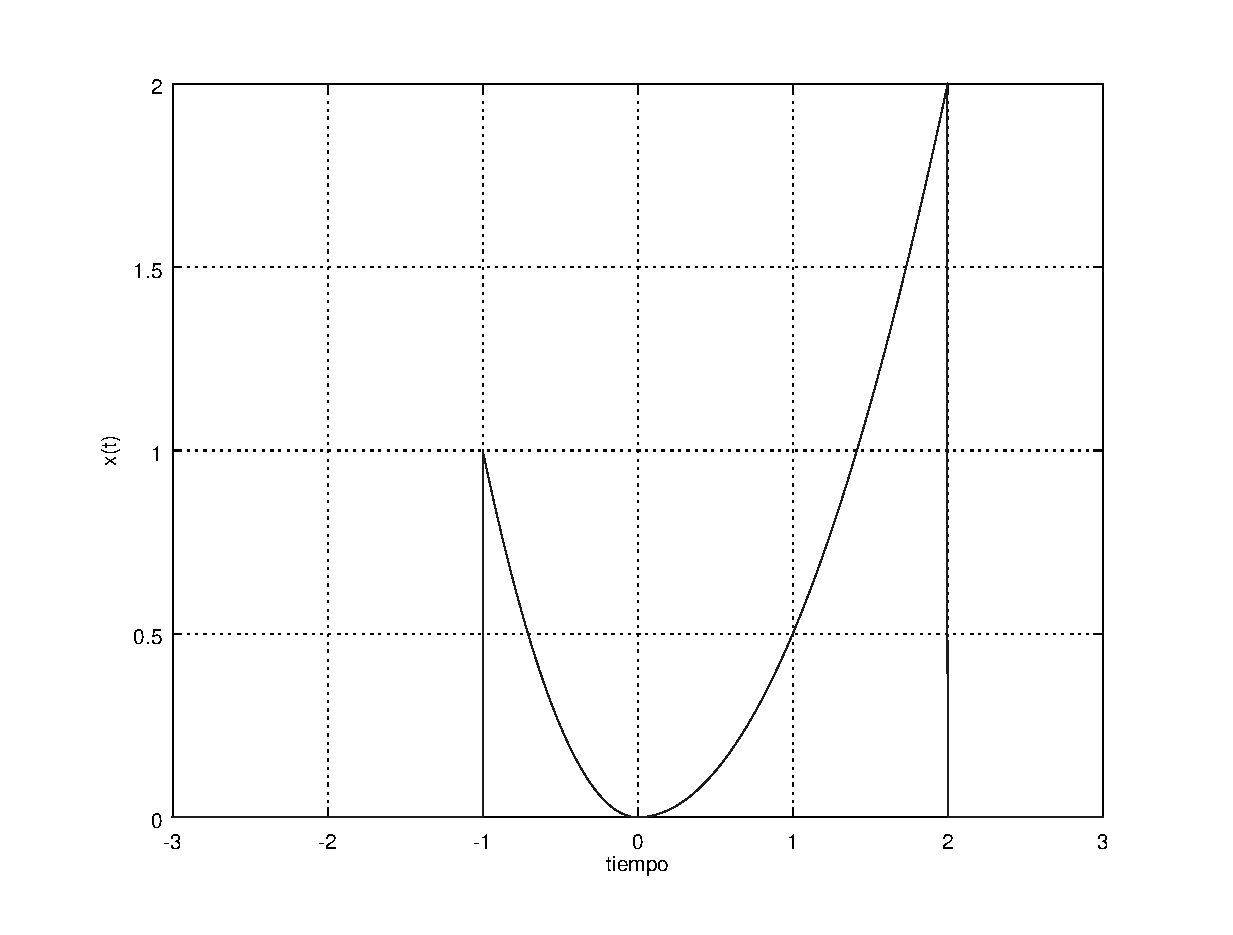
\includegraphics[width=1\linewidth]{./Ejercicio1/Aproximacion2b}
        \caption{Multiplicación de ambas señales}
        \label{fig:Aprox2b}
      \end{center}
    \end{subfigure}
    
    \caption{Segunda aproximación a la señal}
    \label{fig:Aprox2}
  \end{center}
\end{figure}


Código en matlab:

\lstinputlisting{./Ejercicio1/aprox2.m}

Ahora necesitamos generar el valor constante que toma la señal en sus extremos, esto lo podemos generar con la suma de otra señal $\Pi$ invertida en amplitud y desplazada hacia arriba una unidad.\\

\begin{figure}[H]
  \begin{center}
    
    \begin{subfigure}{0.5\textwidth}
      \begin{center}
        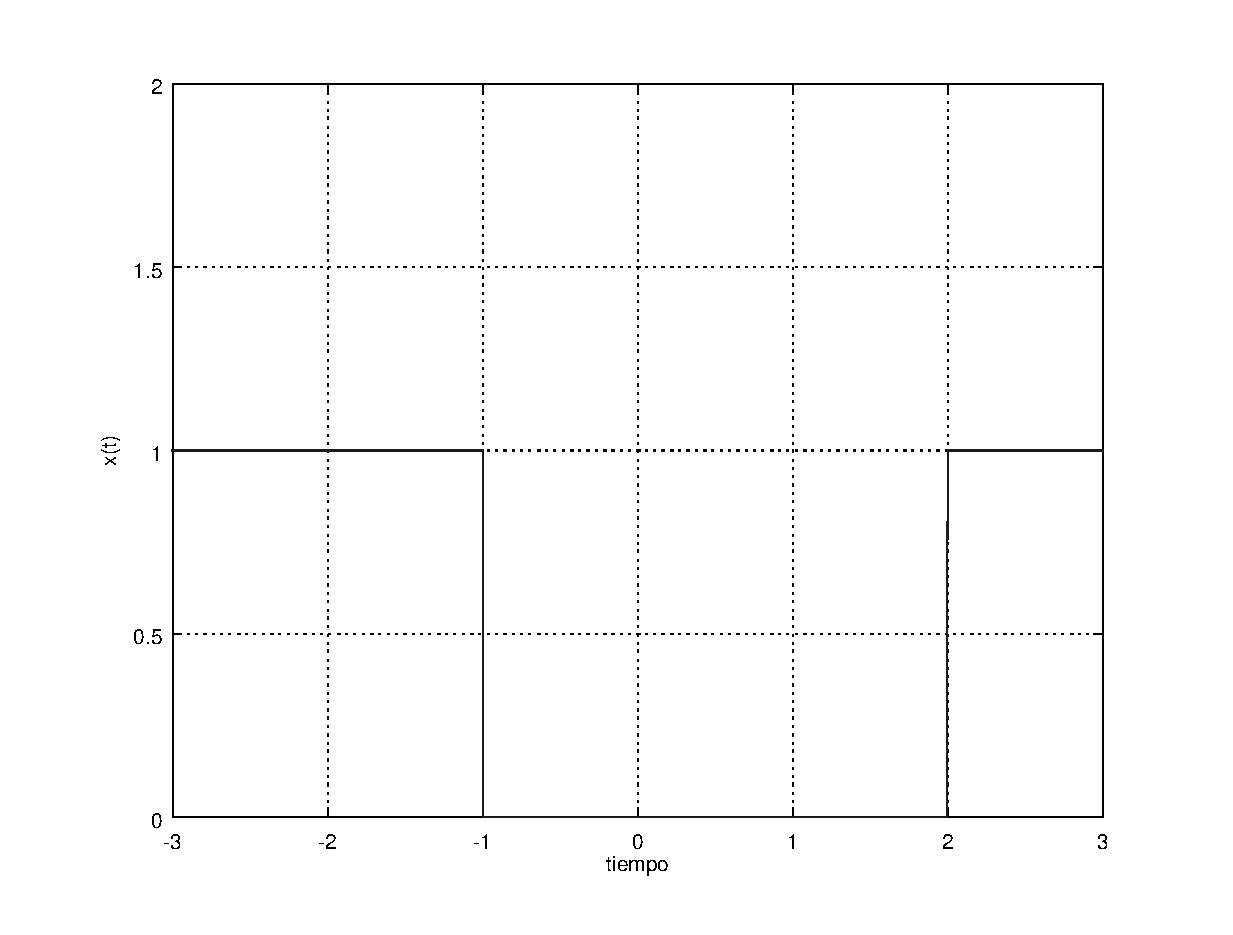
\includegraphics[width=1\linewidth]{./Ejercicio1/Aproximacion3a}
        \caption{Señal $\Pi(t)$ expandida, retrasada, invertida en amplitud y trasladada una unidad hacia arriba}
        \label{fig:Aprox3a}
      \end{center}
    \end{subfigure}%    
    \begin{subfigure}{0.5\textwidth}
      \begin{center}
        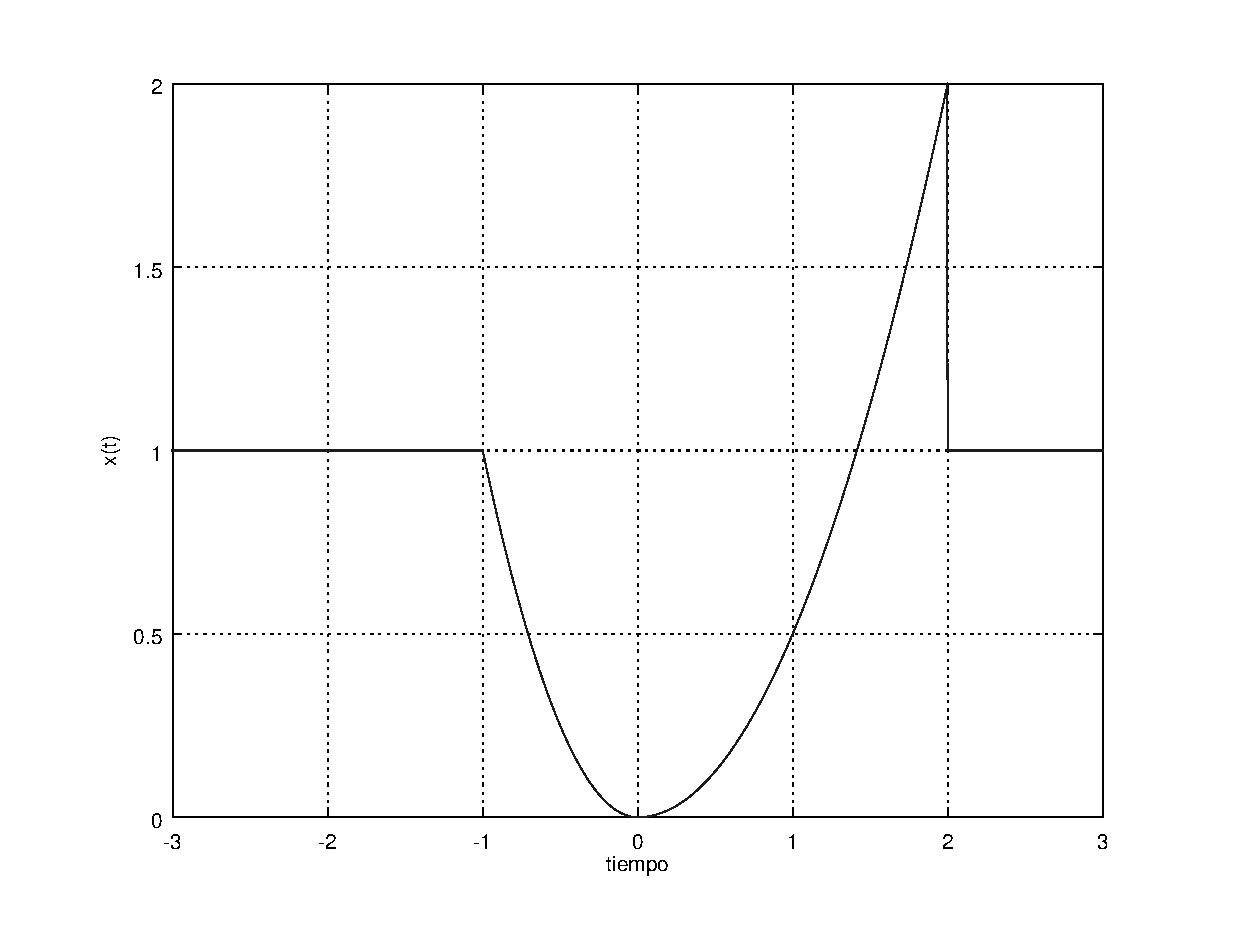
\includegraphics[width=1\linewidth]{./Ejercicio1/Aproximacion3b}
        \caption{Suma de ambas señales}
        \label{fig:Aprox3b}
      \end{center}
    \end{subfigure}
    
    \caption{Tercera aproximación a la señal}
    \label{fig:Aprox3}
  \end{center}
\end{figure}
Así la señal de la \texttt{figura 1.4b} es la señal expresada como funciones singulares.

\[ x(t) = \left[2u_{-3}\left(t\right)+u_{-3}\left(t\right)\right]\times\Pi\left(\frac{t-\frac{1}{2}}3\right)-\left(\Pi\left(\frac{t-\frac{1}{2}}3\right)-1\right) \] 

Código en matlab:

\begin{lstlisting}
function x = x1(t)
 x = ( ( 2*pu(-t) + pu(t) ) .* rect( (t.-0.5) ./ 3 ) ) .- ( rect( (t.-0.5) ./ 3 ) .- 1);

t = -15 : 0.005 : 15;
plot(t,x1(t));
axis([-3,3,0,2]);
grid();
xlabel("tiempo");
ylabel("x(t)"); 
\end{lstlisting}



\section{Ejercicio 2}
Si $x\left(t\right)$ es la que obtuvo en el Ejercicio 1, obtenga las siguientes señales:

\begin{enumerate}
  \item $x\left(\frac{t}{4}\right)$\\
  \newline Para esta gráfica la señal sufre una transformación en el tiempo, como el valor del coeficiente $\alpha$ de $t$ es igual a $\frac{1}{4}$, la señal se verá expandida en un factor inverso, es decir, la veremos cuatro veces más ancha. Esto se notará más en los limites de la parábola, los cuales irán de -4 a 8. Las funciones siempre van a tener su valor mínimo en 0, para cualquier transformación en el tiempo, además, durante la transformación la función $\Pi(t)$ sigue cortando en el mismo rango a las parábolas, por lo que la amplitud no se ve modificada.

    \begin{figure}[H]
      \begin{center}
        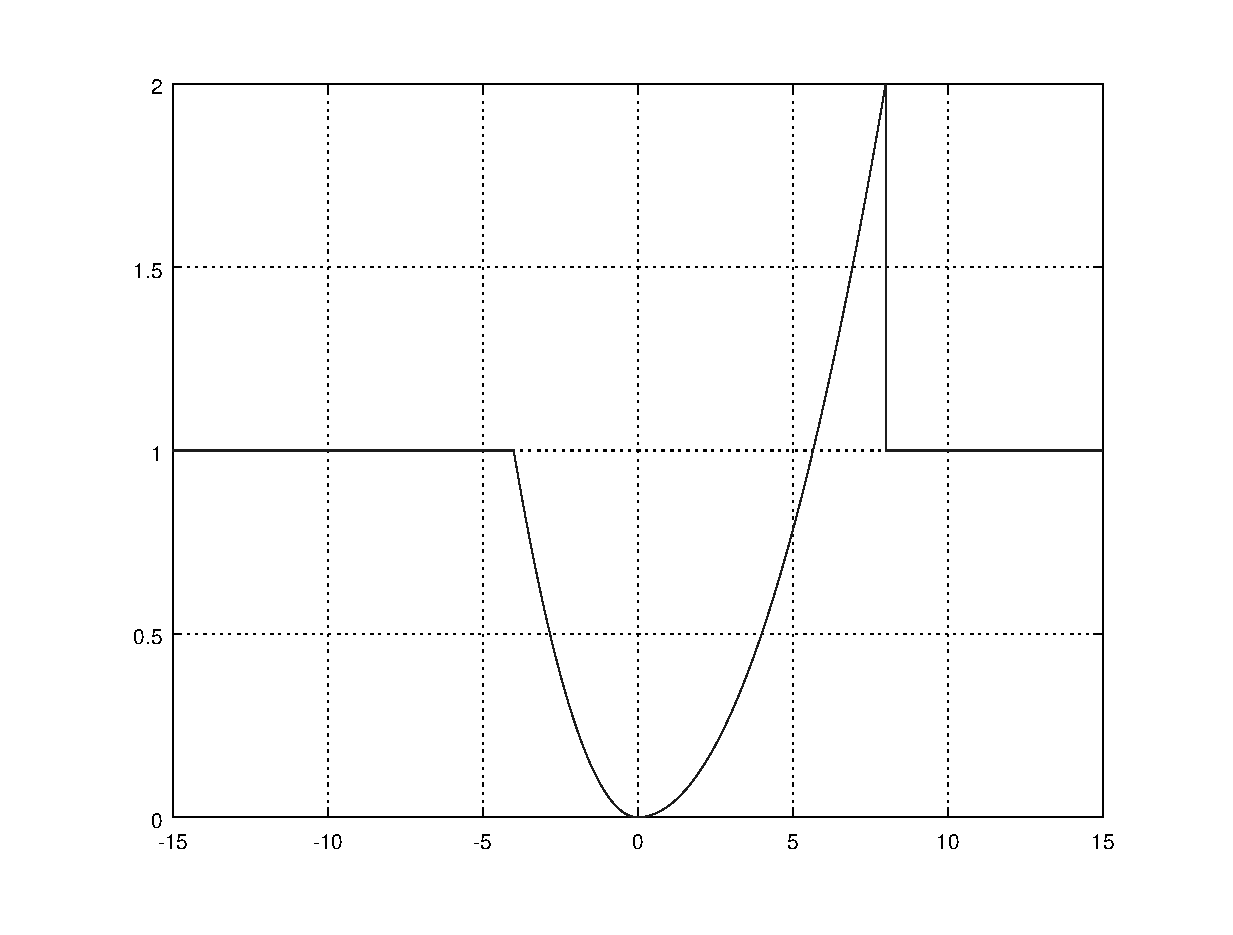
\includegraphics[width=0.5\textwidth]{./Ejercicio2/IncisoA}
        \caption{Señal expandida 4 veces}
        \label{fig:IncisoA}
      \end{center}
    \end{figure}
    
Código en Matlab:
    \lstinputlisting{./Ejercicio2/incisoa.m}

  \item $x\left(2t-\frac{1}{4}\right)$\\
    \newline Para nueva señal, la señal original es contraída 2 veces su ancho original y adelantada en $\frac{1}{8}$ unidad. Esto lo podemos ver mejor si reescribimos la función anterior como $x\left(2\left(t-\frac{1}{8}\right)\right)$ De forma análoga al inciso anterior, la amplitud no se modifica.

    \begin{figure}[H]
      \begin{center}
        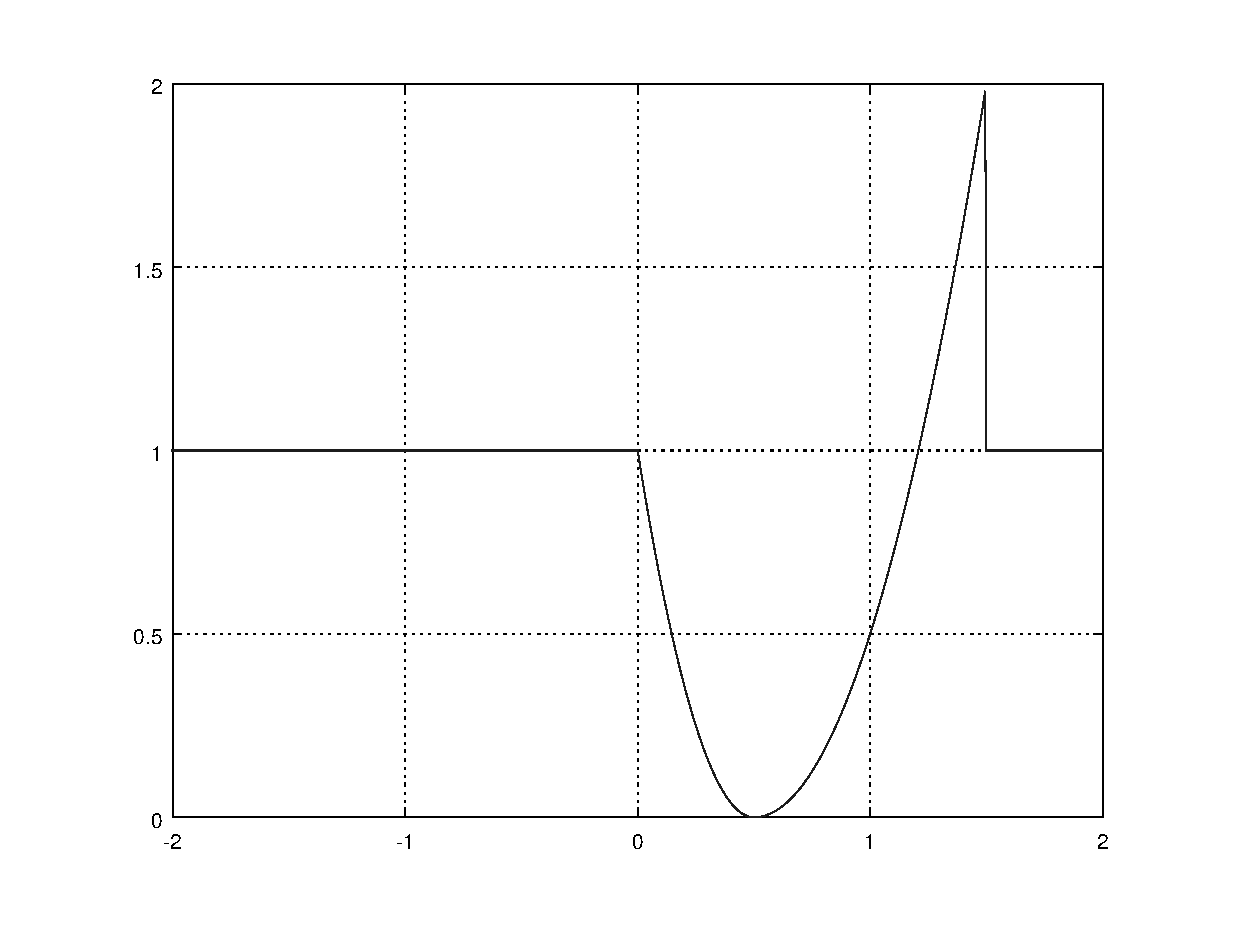
\includegraphics[width=0.5\textwidth]{./Ejercicio2/IncisoB}
        \caption{Señal contraída 2 veces y adelantada $\frac{1}{8}$ de unidad}
        \label{fig:IncisoB}
      \end{center}
    \end{figure}
    
Código en Matlab:
    \lstinputlisting{./Ejercicio2/incisob.m}
    
  \item $x\left(-\frac{t}{4}-1\right)$\\
  \newline Si reescribimos esta señal como $x\left(-\frac{\left(t+4\right)}{4}\right)$ nos es más fácil ver que es una la señal retrasada 4 unidades, expandida 4 veces y luego invertida en el tiempo. Transformar la señal en este orden es equivalente a primero expandir la señal 4 veces y luego adelantarla 4 unidades. Nuevamente la amplitud no se ve afectada.

    \begin{figure}[H]
      \begin{center}
        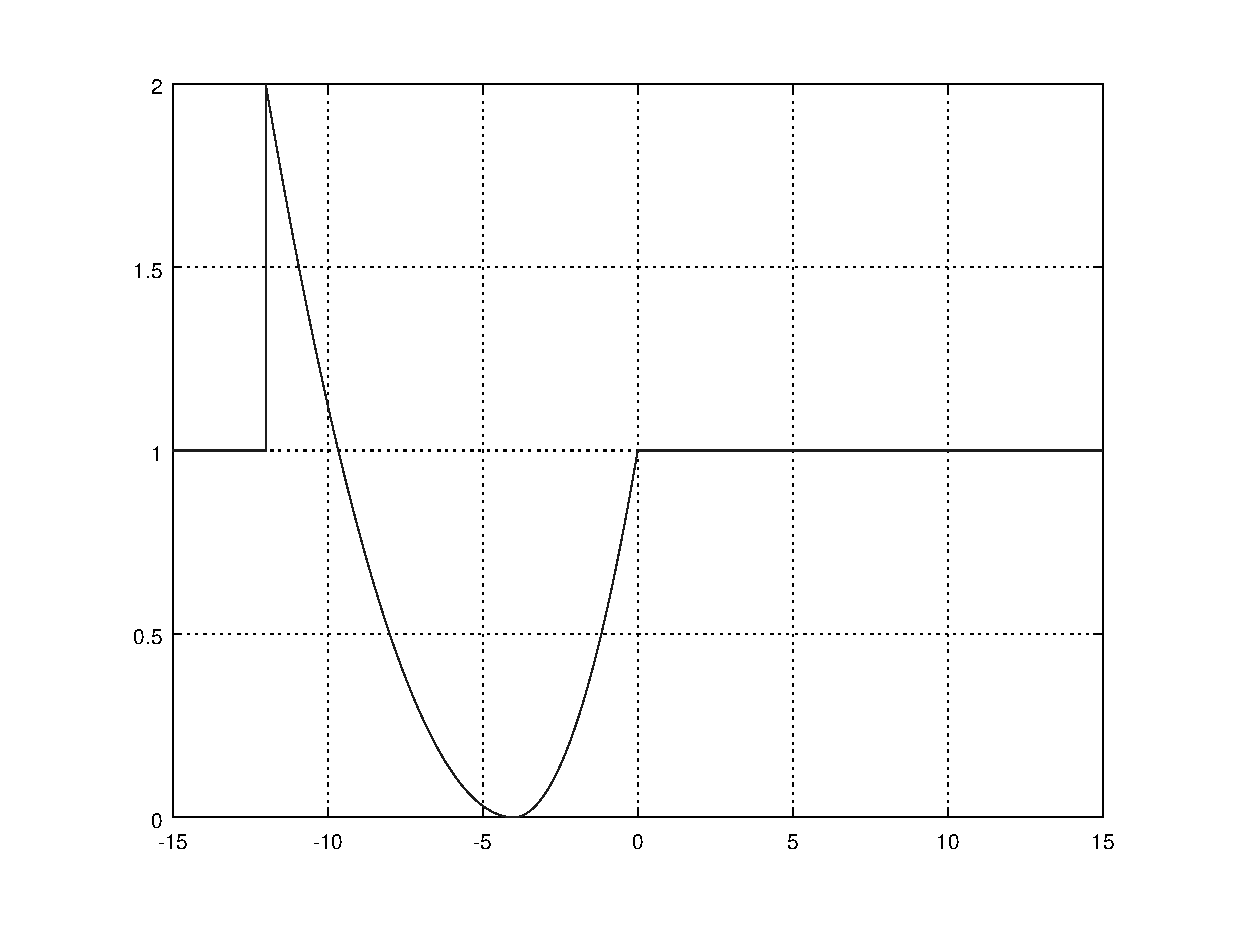
\includegraphics[width=0.5\textwidth]{./Ejercicio2/IncisoC}
        \caption{Señal expandida 4 veces, invertida en el tiempo y retrasada 4 unidades}
        \label{fig:IncisoC}
      \end{center}
    \end{figure}
    
Código en Matlab:
    \lstinputlisting{./Ejercicio2/incisoc.m}
    \newpage

  \item $x\left(\frac{t}{4}+\frac{1}{4}\right)$\\
  \newline Nuevamente reescribamos la señal para ver de forma más clara el comportamiento que presenta: $x\left(\frac{t+1}{4}\right)$. En esta nueva expresión podemos ver que la señal es adelantada 1 unidad y luego expandida 4 unidades. De nuevo, la amplitud original se conserva.
    \begin{figure}[H]
      \begin{center}
        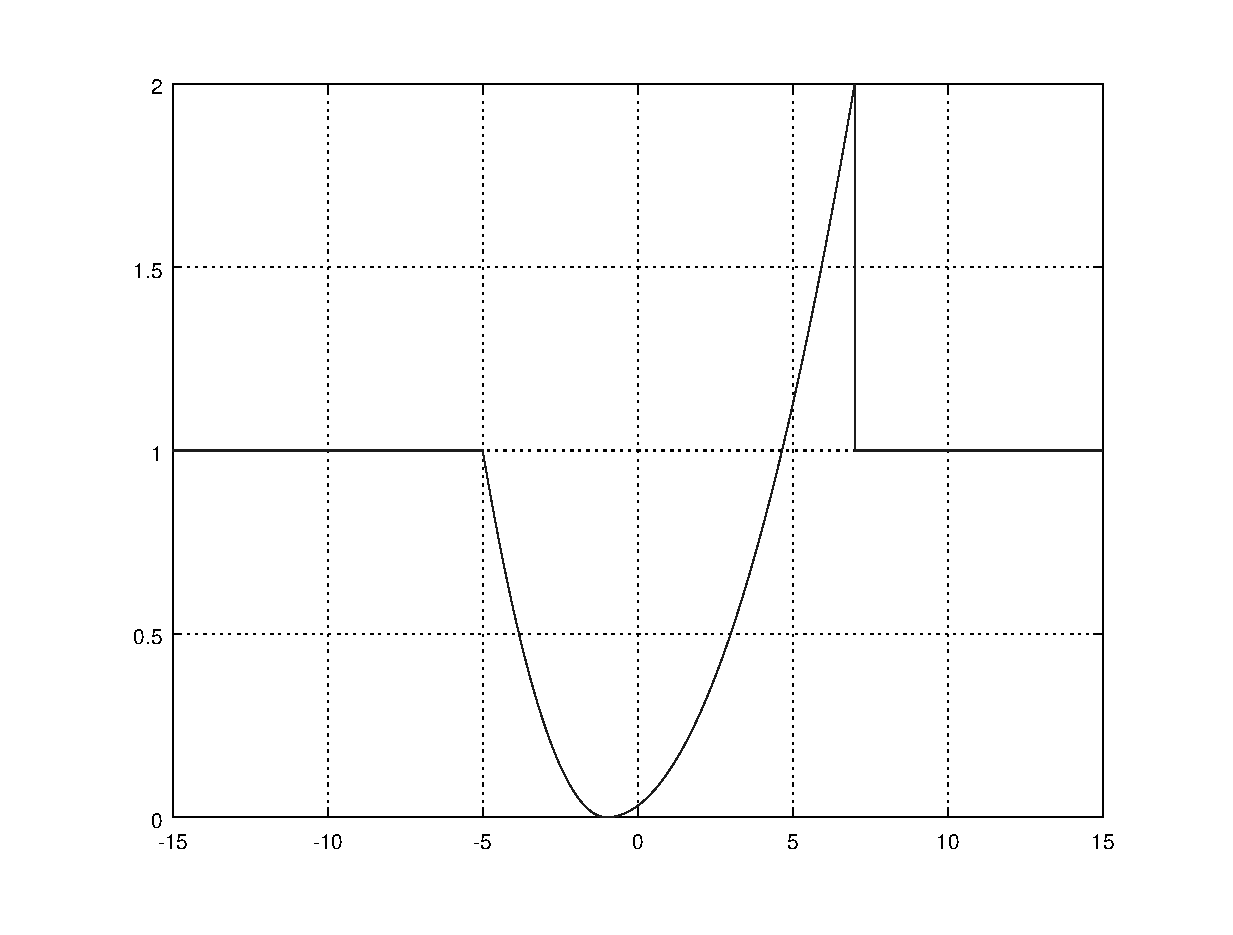
\includegraphics[width=0.5\textwidth]{./Ejercicio2/IncisoD}
        \caption{Señal expandida 4 veces y retrasada 1 unidad}
        \label{fig:IncisoD}
      \end{center}
    \end{figure}
    
Código en Matlab:
    \lstinputlisting{./Ejercicio2/incisod.m}
    
\end{enumerate}
\section{Ejercicio 3}
\begin{enumerate}
\item Determine la señal Par\{x(t)\} y diga si es periódica.
\[ Par\left\{ x\left( t \right)  \right\} =\frac { 1 }{ 2 } \left[ \left( 2u_{ -3 }\left( -t \right) +{ u }_{ -3 }\left( t \right)  \right) \Pi \left( \frac { t-\frac { 1 }{ 2 }  }{ 3 }  \right) -\left( \Pi \left( \frac { t-\frac { 1 }{ 2 }  }{ 3 }  \right) -1 \right) \right.\]
\[ \qquad \left.  + \left( 2u_{ -3 }\left( t \right) +{ u }_{ -3 }\left( -t \right)  \right) \Pi \left( \frac { -\left( t+\frac { 1 }{ 2 }  \right)  }{ 3 }  \right) -\left( \Pi \left( \frac { -\left( t+\frac { 1 }{ 2 }  \right)  }{ 3 }  \right) -1 \right) \right] \]
La señal no es periódica.
\begin{figure}[H]
  \begin{center}
    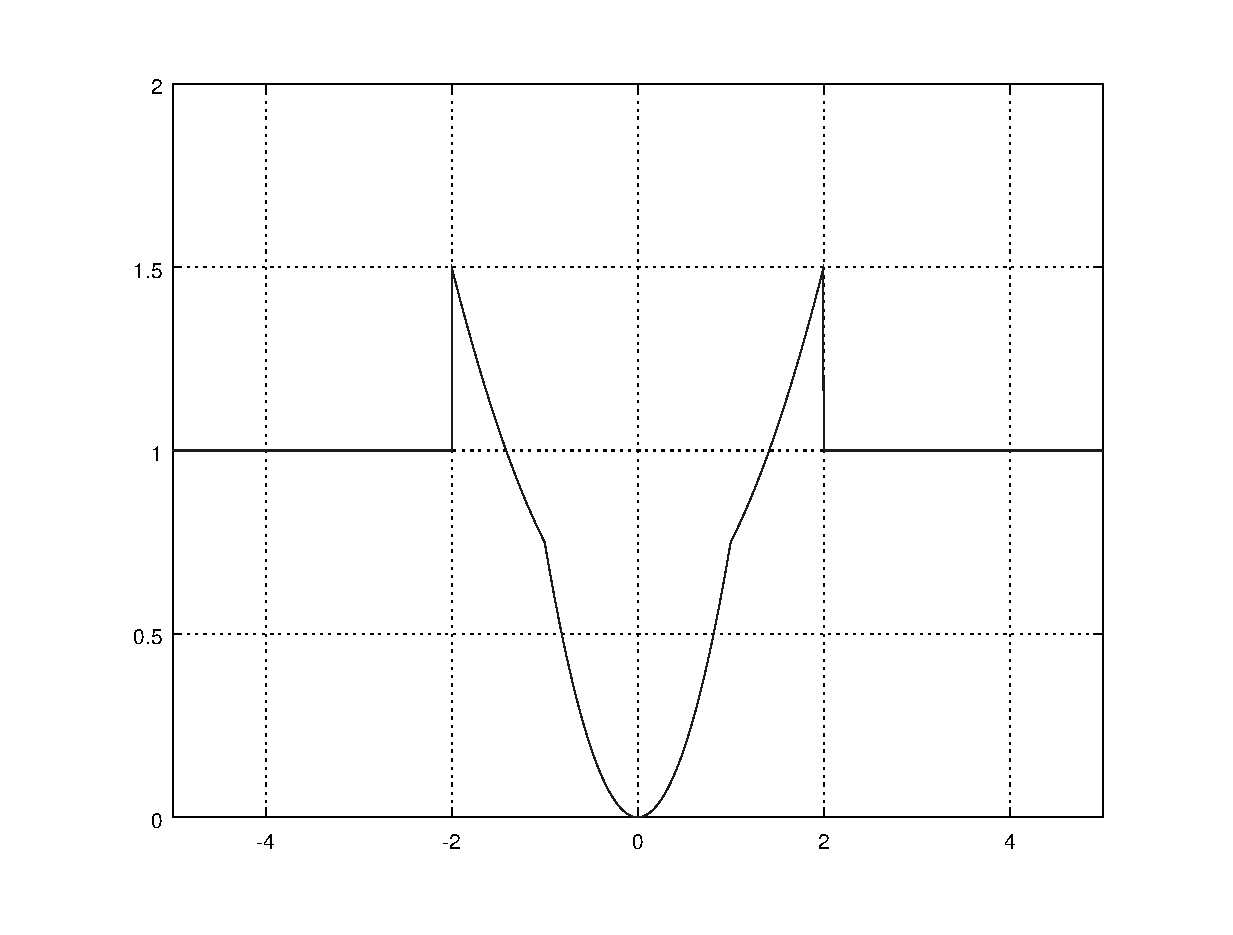
\includegraphics[width=0.5\textwidth]{./Ejercicio3/Par}
    \caption{Par\{x(t)\}}
    \label{fig:Par}
  \end{center}
\end{figure}
Código en Matlab:
    \lstinputlisting{./Ejercicio3/grafpar.m}
\item Determine la señal Impar\{x(t)\} 
\[ Impar\left\{ x\left( t \right)  \right\} =\frac { 1 }{ 2 } \left[ \left( 2u_{ -3 }\left( -t \right) +{ u }_{ -3 }\left( t \right)  \right) \Pi \left( \frac { t-\frac { 1 }{ 2 }  }{ 3 }  \right) -\left( \Pi \left( \frac { t-\frac { 1 }{ 2 }  }{ 3 }  \right) -1 \right) \right.\]
\[ \qquad \left.  - \left( 2u_{ -3 }\left( t \right) +{ u }_{ -3 }\left( -t \right)  \right) \Pi \left( \frac { -\left( t+\frac { 1 }{ 2 }  \right)  }{ 3 }  \right) +\left( \Pi \left( \frac { -\left( t+\frac { 1 }{ 2 }  \right)  }{ 3 }  \right) -1 \right) \right] \]
\begin{figure}[H]
  \begin{center}
    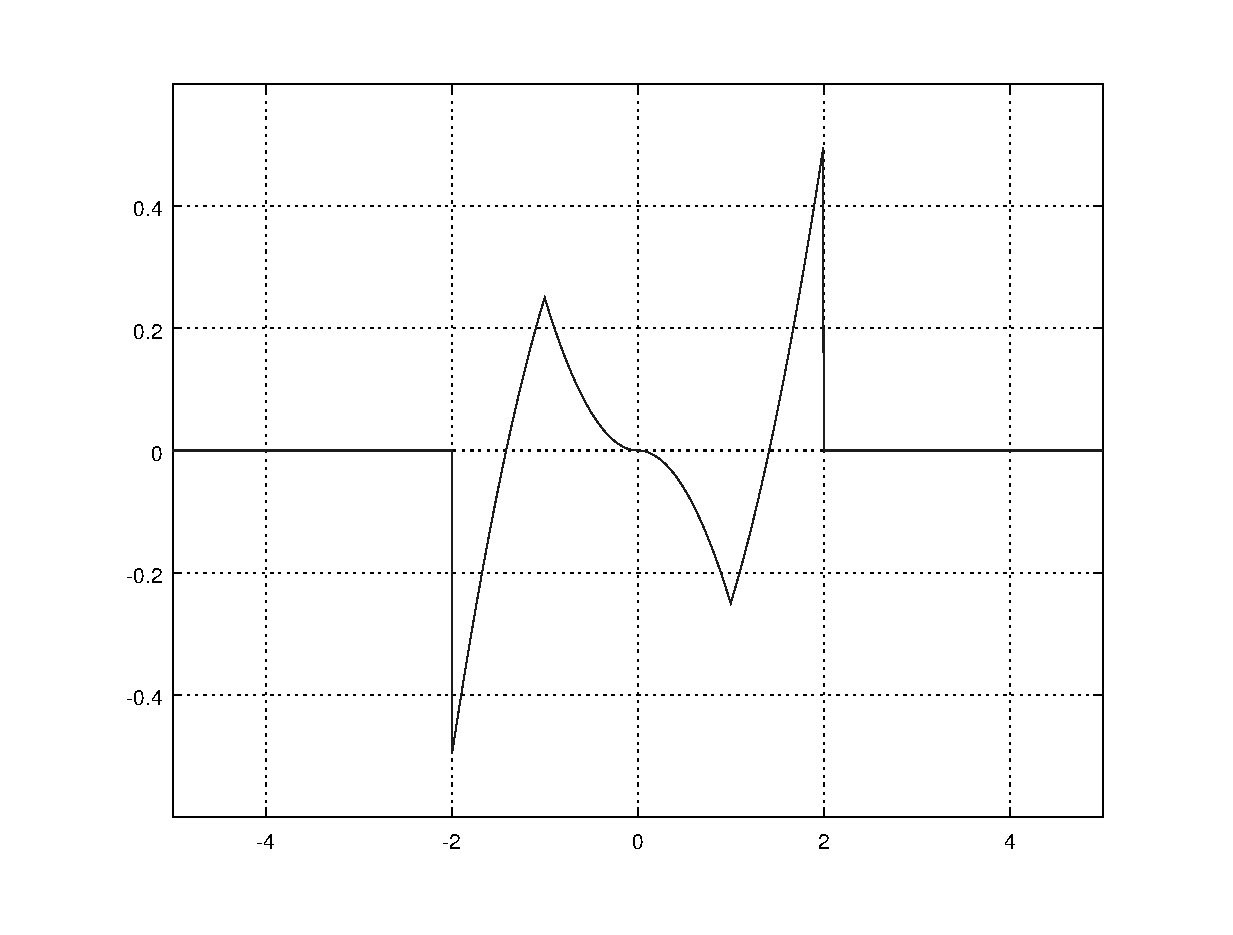
\includegraphics[width=0.5\textwidth]{./Ejercicio3/Impar}
    \caption{Impar\{x(t)\}}
    \label{fig:Impar}
  \end{center}
\end{figure}
Código en Matlab:
    \lstinputlisting{./Ejercicio3/grafimpar.m}
\item Encuentra Par\{x(t)\}+Impar\{x(t)\}
$\qquad Par\{x(t)\}+Impar\{x(t)\} = x(t)$
\begin{figure}[H]
  \begin{center}
    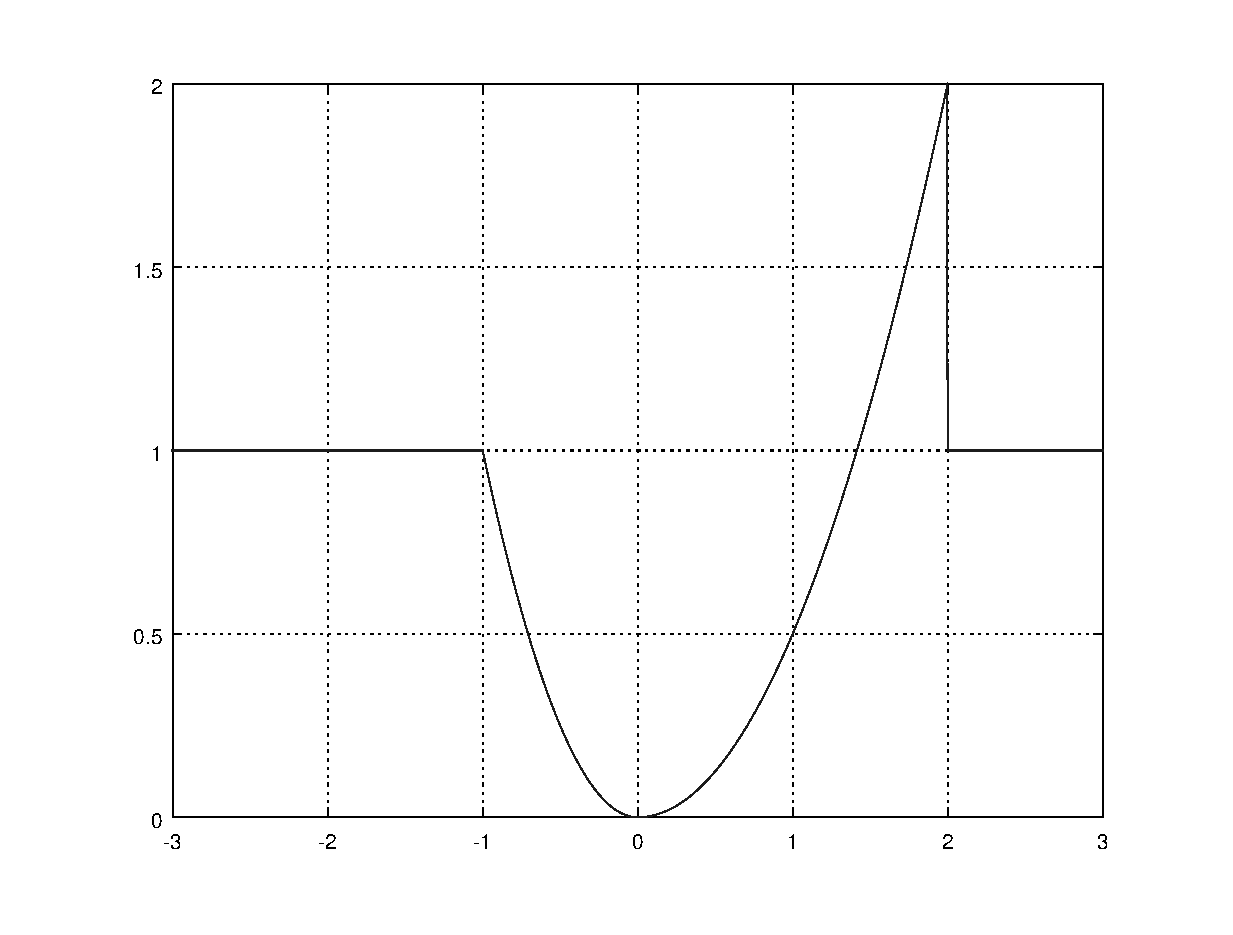
\includegraphics[width=0.5\textwidth]{./Ejercicio3/ParImpar}
    \caption{Par\{x(t)\}+Impar\{x(t)\}}
    \label{fig:ParImpar}
  \end{center}
\end{figure}
Código en Matlab:
    \lstinputlisting{./Ejercicio3/grafparimpar.m}
\end{enumerate}
\section{Ejercicio 4}
Determine si los siguientes sistemas de tiempo continuo son o no lineales, variantes en el tiempo, causales, con memoria y estables. Justifique su respuesta.
\begin{enumerate}
  \item  $ y\left[n\right]\;=\;\left\{\begin{array}{lc}
                                     1&n\geq0 \\
                                     0&n<0 \\ 
                                   \end{array}\right. \quad \forall\;x\left[n\right]
$\\
    \begin{itemize}
      \item Lineal o no lineal\\
$ y_1[n] = \;\left\{\begin{array}{lc}
                      1&n\geq0 \\
                      0&n<0 \\ 
                    \end{array}\right. \quad \forall\;x_1\left[n\right]\\
  y_2[n] = \;\left\{\begin{array}{lc}
                      1&n\geq0 \\
                      0&n<0 \\ 
                    \end{array}\right. \quad \forall\;x_2\left[n\right]\\
  x_3[n] = x_1[n]+x_2[n]\\
  y_3[n] = \;\left\{\begin{array}{lc}
                      1&n\geq0 \\
                      0&n<0 \\ 
                    \end{array}\right. \quad \forall\;x_3\left[n\right]\\
$
\newline Este sistema no es lineal.
      \item Variante o invariante en el tiempo\\
$
  y[n-n_0] = \;\left\{\begin{array}{lc}
                      1 & n\geq n_0 \\
                      0 & n < n_0 \\ 
                    \end{array}\right. \quad \forall\;x\left[n-n_0\right] \qquad$ condición de invariabilidad\\
$ x_1=[n-n_0] $\\
$ y[n-n_0] = \;\left\{\begin{array}{lc}
                      1 & n-n_0 \geq 0\\
                      0 & n-n_0 < 0 \\ 
                    \end{array}\right. \quad \forall\;x\left[n-n_0\right]$\\
$
  y[n-n_0] = \;\left\{\begin{array}{lc}
                      1 & n\geq n_0 \\
                      0 & n < n_0 \\ 
                    \end{array}\right. \quad \forall\;x\left[n-n_0\right]$\\
\newline Este sistema es invariante en el tiempo.\\
      \item Causalidad\\
      $ y[0] = 1\; \forall\;x[0] $\\
      $ y[-1] = 0\; \forall\; x[-1] $\\
      $ y[1] = 1\; \forall\; x[1] $\\
\newline Este sistema no depende de valores futuros o pasados de la señal, por lo que es un sistema causal o no anticipativo.

      \item Con o sin memoria\\
      Al ser un sistema causal, éste no tiene memoria.
      
      \item Estabilidad\\
      Este sistema siempre tendrá el valor de 1 para cualquier valor mayor o igual que cero que tome la señal, o cero en otro caso por lo que este sistema siempre tendrá una salida acotada, entre 0 y 1 sin importar si la señal de entrada es estable o no. Podemos entonce decir que es un sistema estable BIBO.
    \end{itemize}
    
  \item $y(t)=sen(x(t+1)) $
  \begin{itemize}
    \item Lineal o no lineal\\
$ y_1(t)\;=\;sen(x_1(t+1))\\
  y_2(t)\;=\;sen(x_2(t+1))\\
  x_3(t)\;=\;x_1(t)+x_2(t)\\
  y_3(t)\;=\;sen(x_3(t+1))\\
  y_3(t)\;=\;sen(x_1(t+1)+x_2(t+1))\;\neq\;sen(x_1(t+1))+sen(x_2(t+1))
$\\
  \newline Este sistema no es lineal por que no cumple la propiedad de aditividad.

  \item Variante o invariante en el tiempo\\
$ y(t-t_0)\;=\;sen(x(t-t_0+1)) \qquad $ Condición de invariabilidad\\
$ x_1(t)=x(t-t_0) \qquad $ Proponemos una nueva señal, desplaza en el tiempo \\ 
$ y_1(t)=sen(x_1(t+1)) $\\
$ y_1(t)=sen(x(t-t_0+1)) $\\
  \newline  
  Este sistema es invariante en el tiempo por que cumple la condición de invariabilidad\\
  \item Causalidad\\
$y(0)\;=\;sen(x(1))\\
y(-1)\;=\;sen(x(0))\\
y(1)\;=\;sen(x(2))$\\
  \newline
Vemos que el sistema depende de valores futuros de la señal, por lo tanto es un sistema no causal o anticipativo.
  \item Memoria\\
Al depender de valores futuros, este sistema tiene memoria.

  \item Estabilidad\\
La función seno es una función que oscila entre -1 y 1 para cualquier valor de su dominio, por que que cualquier señal, acotada o no, generará una salida acotada. De esto concluimos que la señal es estable BIBO.
  \end{itemize}
\end{enumerate}
\section{Ejercicio 5}

Evalúe las siguientes integrales:
\begin{enumerate}
  \item \[ y(t)=\int_{-\infty }^{\infty }[3\delta (t)+e^{-(t-1)}\delta (t)+cos(2\pi t)\dot{\delta}(t)+e^{-t}\ddot{\delta}(t)]dt \]

  \item \[ y(t)=\int_{0}^{\infty }e^{-(t-1)}\delta (t+10)dt \]

\end{enumerate}
Para la primera ecuación tenemos que usando propiedades de la integral impropia podemos realizar esta descomposición:
\[ y(t)=3\int_{-\infty }^{\infty }\delta (t)dt+\int_{-\infty }^{\infty }e^{-(t-1)}\delta (t)dt+\int_{-\infty }^{\infty }cos(2\pi t)\dot{\delta}(t)dt+\int_{-\infty }^{\infty }e^{-t}\ddot{\delta}(t)dt \]
Recordemos un par de propiedades del impulso y sus derivadas:
\begin{enumerate}
  \item \[ \int_{-\infty}^\infty x\left(t\right)\delta\left(t-t_0\right)\operatorname dx\;=\;x\left(t_0\right) \]
  \item \[ int_a^bx\left(t\right)\delta^{\left(k\right)}\left(t\right)\operatorname dx\;=\;\left(-1\right)^{\left(k\right)}x^{\left(k\right)}\left(0\right); \qquad para \;a<0,\;b>0, \;x^k\left(t\right) \quad continua\;en\;t=0 \]
\end{enumerate}
Con esto podemos decir que:
\[ y\left(t\right) = \left(3+\;e^{-\left(t-1\right)}+cos\left(2\pi t\right)\delta\left(t\right)+\left(-1\right)\dot{e^{-t}}\right)\left|\begin{array}{l}\\t=0\end{array}\right. \]
\[ y\left(t\right) = \left(3+\;e^{-\left(t-1\right)}+cos\left(2\pi t\right)\delta\left(t\right)+{e^{-t}}\right)\left|\begin{array}{l}\\t=0\end{array}\right. \]
Evaluando $t=0$
\[ y\left(t\right) = \left(3+\;e+cos\left(0\right)+e^0\right) \]
\[ y\left(t\right) = \left(3+\;e+1+1\right) \]
\[ y\left(t\right) = 5+e \]\\
Para la segunda integral tendríamos que:
\[ y\left(t\right)= e^{-\left(t-1\right)}\delta\left(t+10\right)\left|\begin{array}{l}\\t=-10\end{array}\right. \]
Pero el intervalo en el que debemos integrar es $\left(0,\infty\right)$, dado que $\delta\left(t\right) = 0 \; \forall \; t \neq -10$ tenemos que:
% Evaluando $t=-10$
% \[ y\left(t\right)= e\delta\left(10\right) \]
% Como $\delta(t) = 0 \; \forall \; t\neq 0$
\[ y\left(t\right)= 0 \] 
\section{Ejercicio 6}
Grafique las siguientes señales:
\begin{enumerate}
  \item $x(t)=\Pi \left(2t-\frac{1}{2}\right)$\\
  $x(t)=\Pi \left(2\left(t-\frac{1}{4}\right)\right)\quad$ señal adelantada $\frac{1}{4}$ de unidad y comprimida a la mitad.
    \begin{figure}[H]
      \begin{center}
        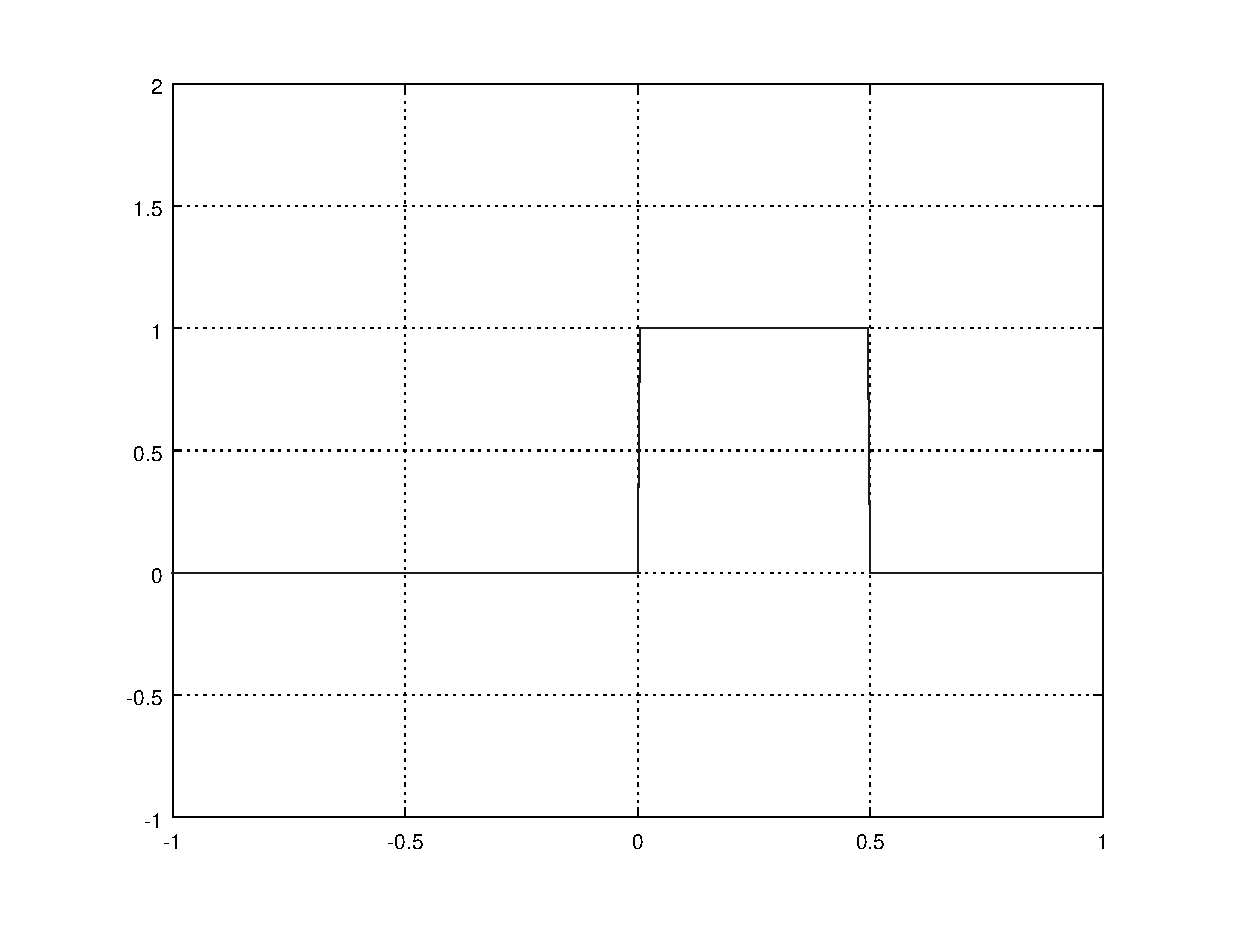
\includegraphics[width=0.45\textwidth]{./Ejercicio6/IncisoA}
        \caption{$x(t)=\Pi \left(2t-\frac{1}{2}\right)$}
        \label{fig:Inciso A}
      \end{center}
    \end{figure}
    Código en Matlab:
    \lstinputlisting{./Ejercicio6/incisoa.m}
  \item $x\left(t\right)=\Pi\left(\frac{t-1}{2}\right)+\Pi\left(t-1\right)\quad$ dos señales $\Pi$, ambas adelantadas 1 unidad, una de ellas expandida al doble de su tamaño original y sumadas.
    \begin{figure}[H]
      \begin{center}
        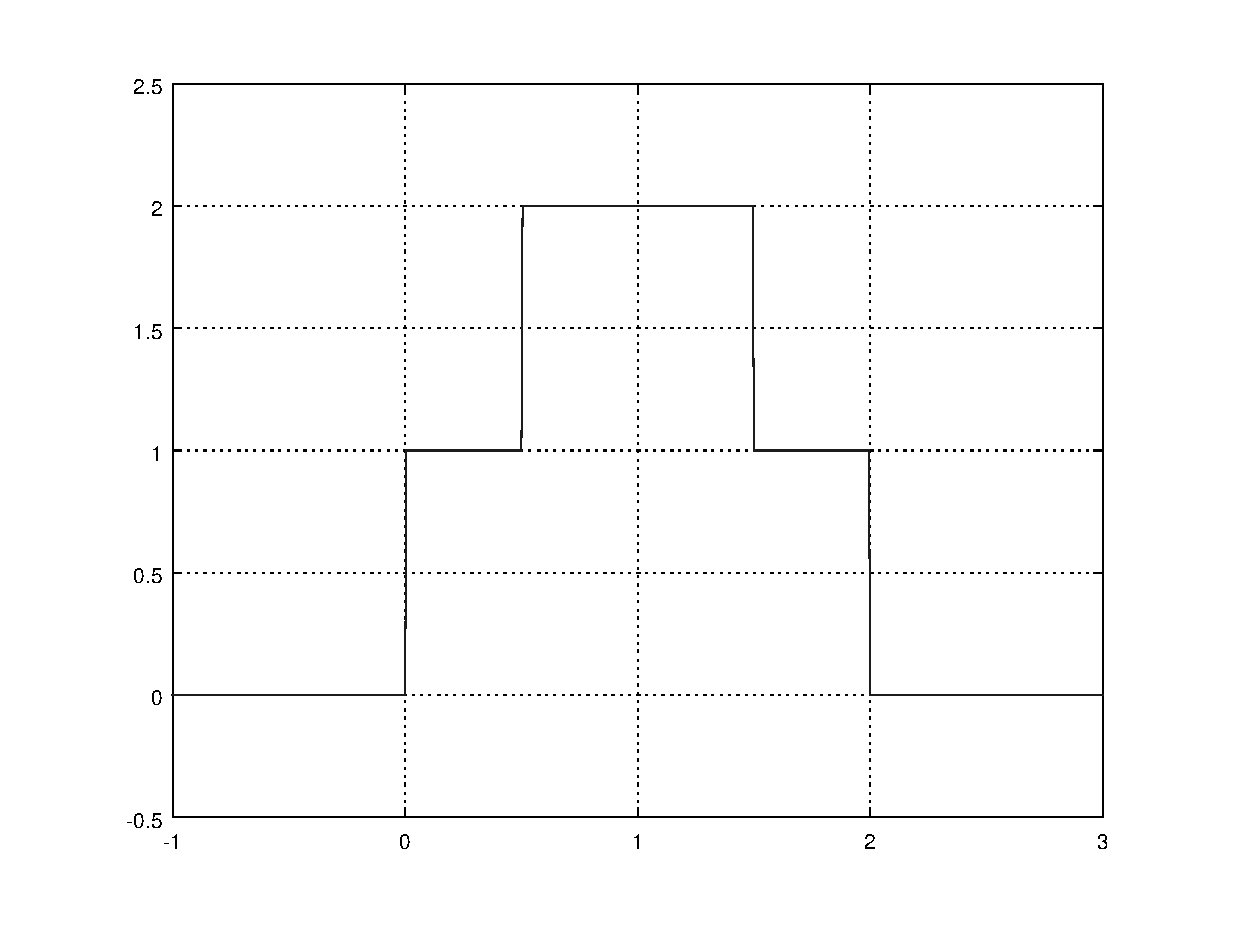
\includegraphics[width=0.45\textwidth]{./Ejercicio6/IncisoB}
        \caption{$x\left(t\right)=\Pi\left(\frac{t-1}{2}\right)+\Pi\left(t-1\right)$}
        \label{fig:Inciso B}
      \end{center}
    \end{figure}
    Código en Matlab:
    \lstinputlisting{./Ejercicio6/incisob.m}
\end{enumerate}

\section{Ejercicio7}
Verifique si la siguiente señal es de energía o de potencia.\\
\[ x(t)=6cos(6\pi t-\pi/3)+4sen(10\pi t) \]
Si recordamos la expresión para calcular la energía de una señal\\
\[ E_{ x }=\int _{ -\infty  }^{ \infty  }{ \left| x(t) \right| ^{ 2 } \partial t} \]
Podemos ver que esta señal por ser periódica y existir en todos los reales, tiene una energía infinita.\\
Si una señal posee una energía infinita se le clasifica como una señal de potencia, por lo tanto esta señal es de potencia.

\begin{figure}[H]
  \begin{center}
    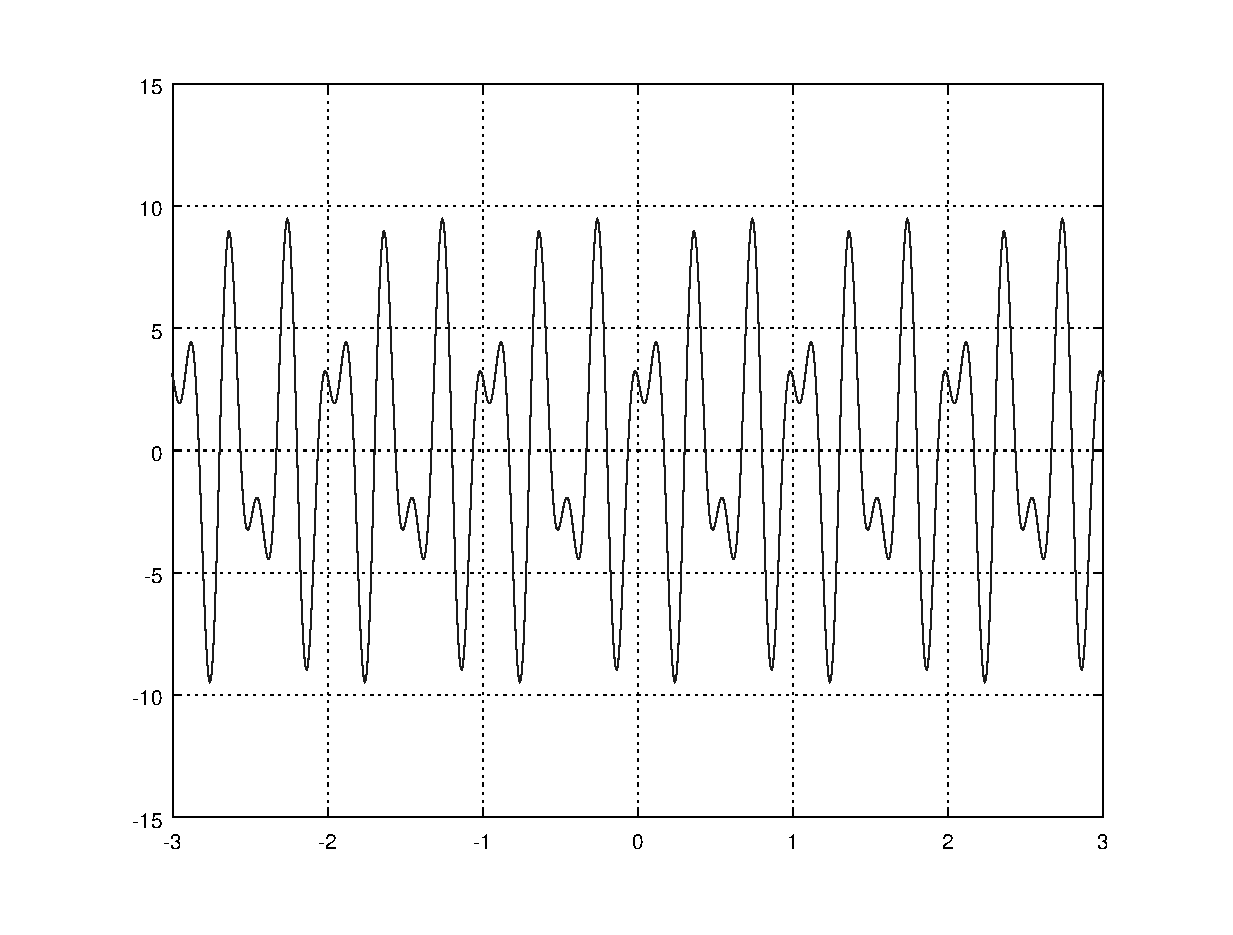
\includegraphics[width=0.85\textwidth]{./Ejercicio7/Potencia}
    \caption{Gráfica de esta señal de potencia}
    \label{fig:Pot}
  \end{center}
\end{figure}

Código en Matlab:
    \lstinputlisting{./Ejercicio7/potencia.m}


% \begin{align}
%   & Ej\text{ }IV: \\ 
%  & x(t)=A\cos (2\pi f_{0}t) \\ 
%  & E_{x}=\int_{-\infty }^{\infty }{\left| x(t) \right|^{2}\partial t=\infty } \\ 
%  & E_{x_{T}}=E_{T}=\int\limits_{{}^{-T}\!\!\diagup\!\!{}_{2}\;}^{{}^{T}\!\!\diagup\!\!{}_{2}\;}{\left| x(t) \right|^{2}\partial t}=\int\limits_{{}^{-T_{0}}\!\!\diagup\!\!{}_{2}\;}^{{}^{T_{0}}\!\!\diagup\!\!{}_{2}\;}{A^{2}\underbrace{\cos ^{2}(2\pi f_{0}t)}_{\text{Par}}\partial t}=2\int\limits_{0}^{{}^{T_{0}}\!\!\diagup\!\!{}_{2}\;}{A^{2}\underbrace{\frac{1+\cos (2\cdot 2\pi f_{0}t)}{2}}_{\cos ^{2}()}\partial t}= \\ 
%  & A^{2}\cdot \left. t+\frac{\sin (2\cdot 2\pi f_{0}t)}{2\cdot 2\pi f_{0}} \right|_{0}^{{}^{T_{0}}\!\!\diagup\!\!{}_{2}\;}=A^{2}\cdot \left( \frac{T_{0}}{2}+\frac{\sin \left( 2\cdot 2\pi f_{0}{}^{T_{0}}\!\!\diagup\!\!{}_{2}\; \right)-0}{2\cdot 2\pi f_{0}} \right)\xrightarrow[f_{0}={}^{1}\!\!\diagup\!\!{}_{T_{0}}\;]{}A^{2}\cdot \left( \frac{T_{0}}{2}+\frac{\sin \left( 2\pi  \right)-0}{2\cdot 2\pi f_{0}} \right)= \\ 
%  & E_{T}=\frac{A^{2}}{2}\cdot T_{0} \\ 
% \end{align}

\section{Ejercicio 8}
Capture al menos dos señales físicas reales y preséntalas en una  gráfica e identifique el tipo de señal en algún segmento de la misma.
\begin{enumerate}
  \item La primera señal es un silbido humano.
    \begin{figure}[H]
      \begin{center}
        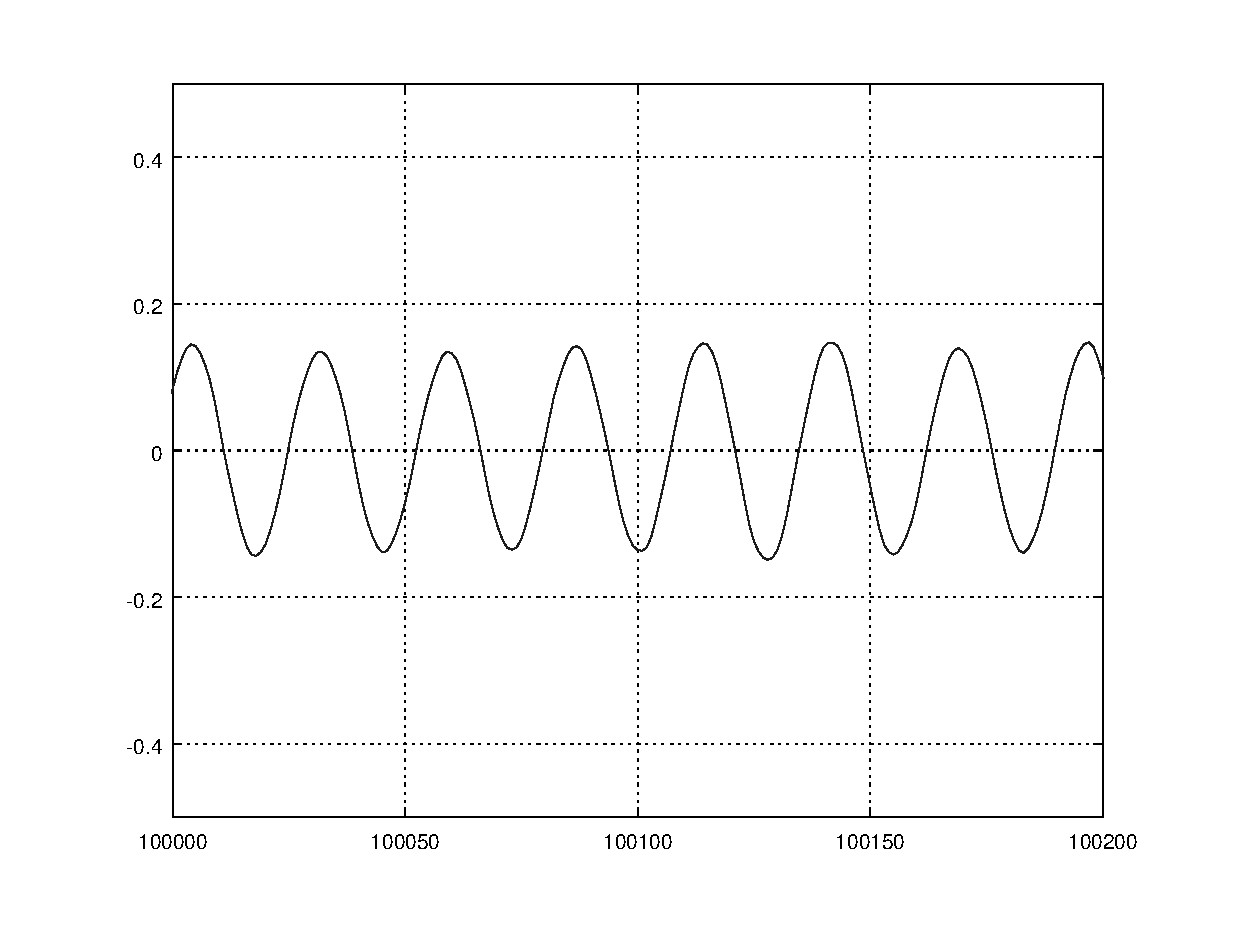
\includegraphics[width=0.4\textwidth]{./Ejercicio8/Silbido}
        \caption{Silbido}
        \label{fig:Slib}
      \end{center}
    \end{figure}
Esta es una señal de tiempo continuo por que la señal puede tomar cualquier valor en cualquier instante de tiempo. \\
Es una señal periódica, ya que (al menos en apariencia a este nivel de acercamiento) se repite en intervalos regulares \\
Es una señal determinista, se puede predecir su comportamiento mediante una función matemática.\\
\newline Código en Matlab
    \lstinputlisting{./Ejercicio8/incisoa.m}
\item La segunda señal corresponde al sonido de las cuerdas de una guitarra acústica.
\begin{figure}[H]
  \begin{center}
    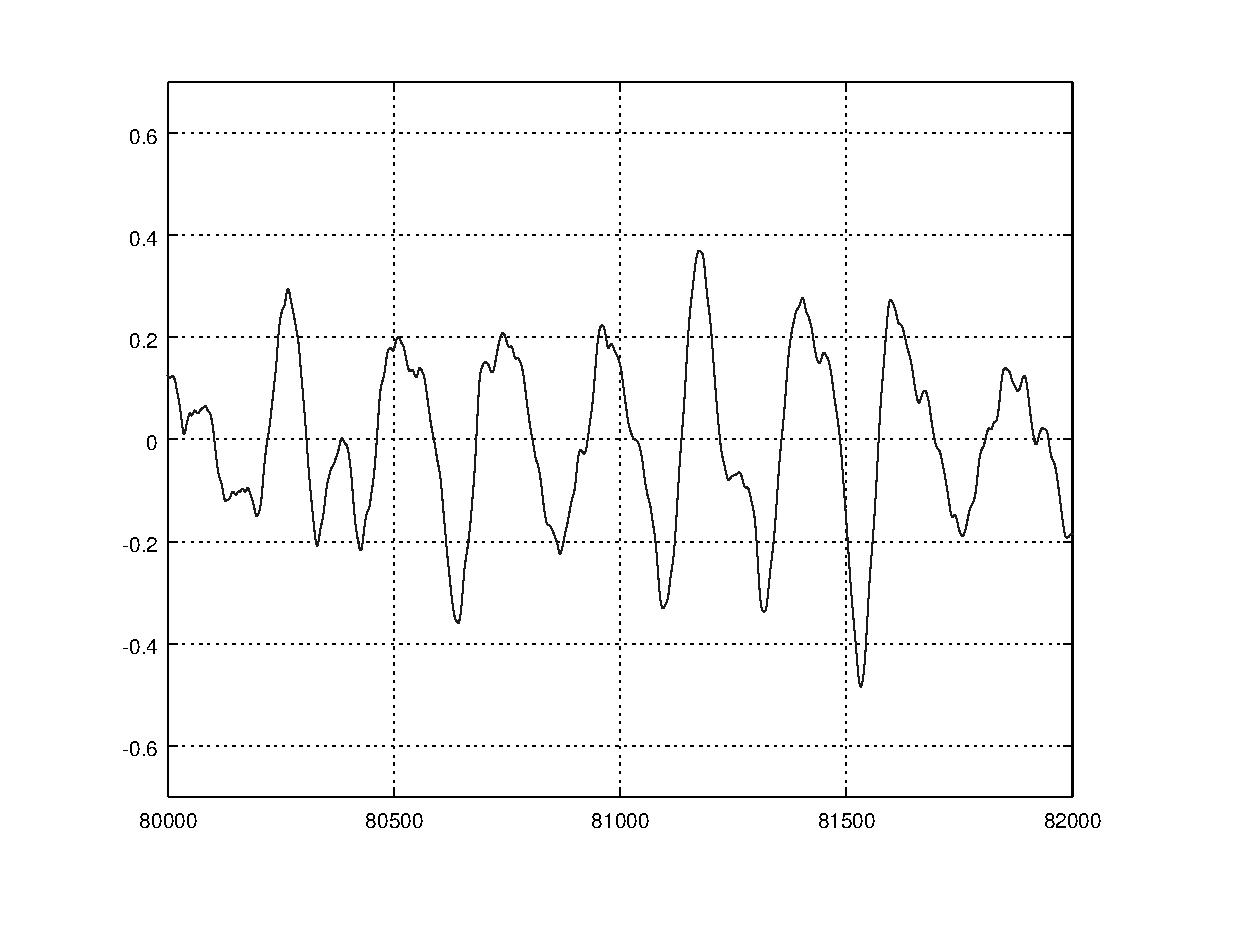
\includegraphics[width=0.4\textwidth]{./Ejercicio8/Guitarra}
    \caption{Sonido de las cuerdas de una guitarra acústica}
    \label{fig:Guitar}
  \end{center}
\end{figure}

Esta es una señal de tiempo continuo por que la señal puede tomar cualquier valor en cualquier instante de tiempo. \\
Es una señal aperiódica, ya que no se repite en intervalos regulares \\
Es una señal aleatoria, ya que no se puede predecir mediante una función matemática.\\
NOTA: Se trató de que el rasgueo de las cuerdas de la guitarra sean igual en tiempo e intensidad, resultó un poco difícil, el mejor de los casos es que hubiera salido igual la gráfica en intervalos regulares, para que la señal sea periódica y determinística.\\
\newline Código en Matlab
    \lstinputlisting{./Ejercicio8/incisoa.m}

\end{enumerate}

\section{Ejercicio 9}

Conexión de sistemas en serie o cascada.\\
\[ S_{1}: y_{1}\left[ n \right]=x_{1}\left[ n \right]+2x_{1}\left[ n-1 \right] \]
\[ S_{2}: y_{2}\left[ n \right]=x_{2}\left[ n+2 \right]+3x_{2}\left[ n \right] \]
S:
\[ x_{2}\left[ n \right]=y_{1}\left[ n \right]=x_{1}\left[ n \right]+2x_{1}\left[ n-1 \right] \]
\[ x_{2}\left[ n+2 \right]=x_{1}\left[ n+2 \right]+2x_{1}\left[ n+2-1 \right] \]
\[ 3x_{2}\left[ n \right]=3x_{1}\left[ n \right]+(3)2x_{1}\left[ n-1 \right] \]
\[ y\left[ n \right]=y_{2}\left[ n \right]=x_{1}\left[ n+2 \right]+2x_{1}\left[ n+1 \right]+3x_{1}\left[ n \right]+6x_{1}\left[ n-1 \right] \]
\[ y\left[ n \right]=6x_{1}\left[ n-1 \right]+3x_{1}\left[ n \right]+2x_{1}\left[ n+1 \right]+x_{1}\left[ n+2 \right] \]\\
Ahora sacaremos su sistema invertido.\\
\[ x_{1}\left[ n \right]=y_{2}\left[ n \right]=x_{2}\left[ n+2 \right]+3x_{2}\left[ n \right] \]
\[ x_{1}\left[ n \right]=x_{2}\left[ n+2 \right]+3x_{2}\left[ n \right] \]
\[ 2x_{1}\left[ n-1 \right]=2x_{2}\left[ n-1+2 \right]+(2)3x_{2}\left[ n-1 \right] \]\\
\[ x\left[ n \right]=x_{2}\left[ n \right]=x_{2}\left[ n+2 \right]+3x_{2}\left[ n \right]+2x_{2}\left[ n+1 \right]+6x_{2}\left[ n-1 \right] \]
\[ x\left[ n \right]=6x_{2}\left[ n-1 \right]+3x_{2}\left[ n \right]+2x_{2}\left[ n+1 \right]+x_{2}\left[ n+2 \right] \]\\
Vemos que el sistema invertido da el mismo resultado.

\section{Ejercicio 10}

Conexión de sistemas en serie o cascada.\\
\[ S_{1}: y_{1}\left[n\right] = nx_{1}\left[n\right] \]
\[ S_{2}: y_{2}\left[n\right] = x_{2}\left[-n-1\right] \]
S:
\[ x_{2}\left[n \right] = y_{1}\left[n\right] = nx_{1}\left[n\right] \]
\[ y\left[n\right] = y_{2}\left[n\right] = x_{2}\left[-n-1\right] \]
\[ y\left[n\right] = \left(-n-1\right)x_{1}\left[-n-1\right] \]
Ahora sacaremos su sistema invertido.\\
\[ x_{1}\left[n\right] = y_{2}\left[n\right]=x_{2}\left[-n-1\right] \]
\[ y\left[n\right] = y_{1}\left[n\right] = nx_{1}\left[n\right] \]
\[ y\left[n\right] = nx_{2}\left[-n-1\right] \]\\
Vemos que al invertir el sistema obtenemos una señal distinta.

\end{document}
